%\documentclass[12pt]{report}
%\usepackage{titlesec}
%\usepackage{etoolbox}
%\usepackage{indentfirst}
%\usepackage{setspace}
%\usepackage{geometry}
%\usepackage{graphicx}
%\usepackage{float}

%\graphicspath{ {Thesis_Images/} }

%\geometry{margin=1in}

%\doublespacing

%\setcounter{secnumdepth}{3}

%\titleformat{\chapter}[block]{\normalfont\bfseries\filcenter}{\thechapter}{1em}{}
%\titleformat{\section}[block]{\normalfont\bfseries}{\thesection}{1em}{}
%\titleformat{\subsection}[block]{\normalfont\bfseries}{\thesubsection}{1em}{}
%\titleformat{\subsubsection}[block]{\normalfont\bfseries}{\thesubsubsection}{1em}{}

%\begin{document}
%%\section{\centering Experimental Setup}
\chapter{Experimental Setup}
%\chapter*{\centering Experimental Setup}
\label{ch:ExpSetup}

\section{The Large Hardon Collider}
The Large Hadron Collider (LHC) accelerates protons and heavy ions in counter rotating beams to near-light speeds. These beams are contained in vacuum tubes that form a circle 26.7 km in circumference and are housed between 50 and 175 m underground, near the France-Switzerland border. The beams cross at four interaction points where four different detectors are located. 

In ideal conditions, each beam contains 2,808 bunches of protons and each bunch contains about 100 billion protons. These bunches are formed from the 16 radio-frequency (RF) cavities located on the beamline. The path and shape of the beam are controlled by about 9,600 magnets. Dipole magnets keep the beams on their circular path, while quadrupole magnets focus the beams. In order for the superconducting dipole magnets to provide a high magnetic field of 8.3 T, they must be kept at 1.9 K with superfluid Helium. 

The design instantaneous luminosity, $\mathcal{L}$, is $10^{-34}\mathrm{cm}^{-2}\mathrm{s}^{-1}$ and only depends on beam parameters:
\begin{equation}
\mathcal{L} = \frac{N_{b}^{2}n_{b}f_{rev}\gamma_{r}}{4\pi\varepsilon_{n}\beta}F
\end{equation}
where $N_{b}$ is the number of particles per bunch, $n_{b}$ is the number of bunches per beam, $f_{rev}$ is the frequency of the revolutions of the beam, $\gamma_{r}$ is the relativistic factor, $\varepsilon_{n}$ is the normalized transverse beam emittance, $\beta$ is the beta function at the collision point and is roughly the width of the beam squared divided by the emittance, and F is the geometric luminosity reduction factor due to the crossing angle at the interaction point~\cite{LHCMachine}. Integrating the instantaneous luminosity with respect to time gives the integrated luminosity:
\begin{equation}
L = \int\mathcal{L}(t)dt
\end{equation}
In 2016, the LHC provided 35.9 $\mathrm{fb}^{-1}$ of integrated luminosity and a similar amount is expected in 2017. This luminosity is delivered with a bunch spacing of 25 ns and a center of mass energy of 13 TeV. To achieve this, electrons are stripped off of Hydrogen atoms by an electric field and the remaining protons are injected into a linear accelerator (LINAC 2) where they reach an energy of 50 MeV. The beam is then sent to the Proton Synchrotron Booster (PSB), which accelerates the protons to 1.4 GeV. Afterwards, the beams are injected into the Proton Synchrotron (PS) where they reach 25 GeV, followed by the Super Proton Synchrotron (PSP) where they are accelerated to 450 GeV. The beams are then accelerated in the main ring to 6.5 TeV. A layout of the acceleration facility can be seen in Figure~\ref{fig:AcceleratorLayout}\cite{LHCLayout}.

\begin{figure}[htbp]
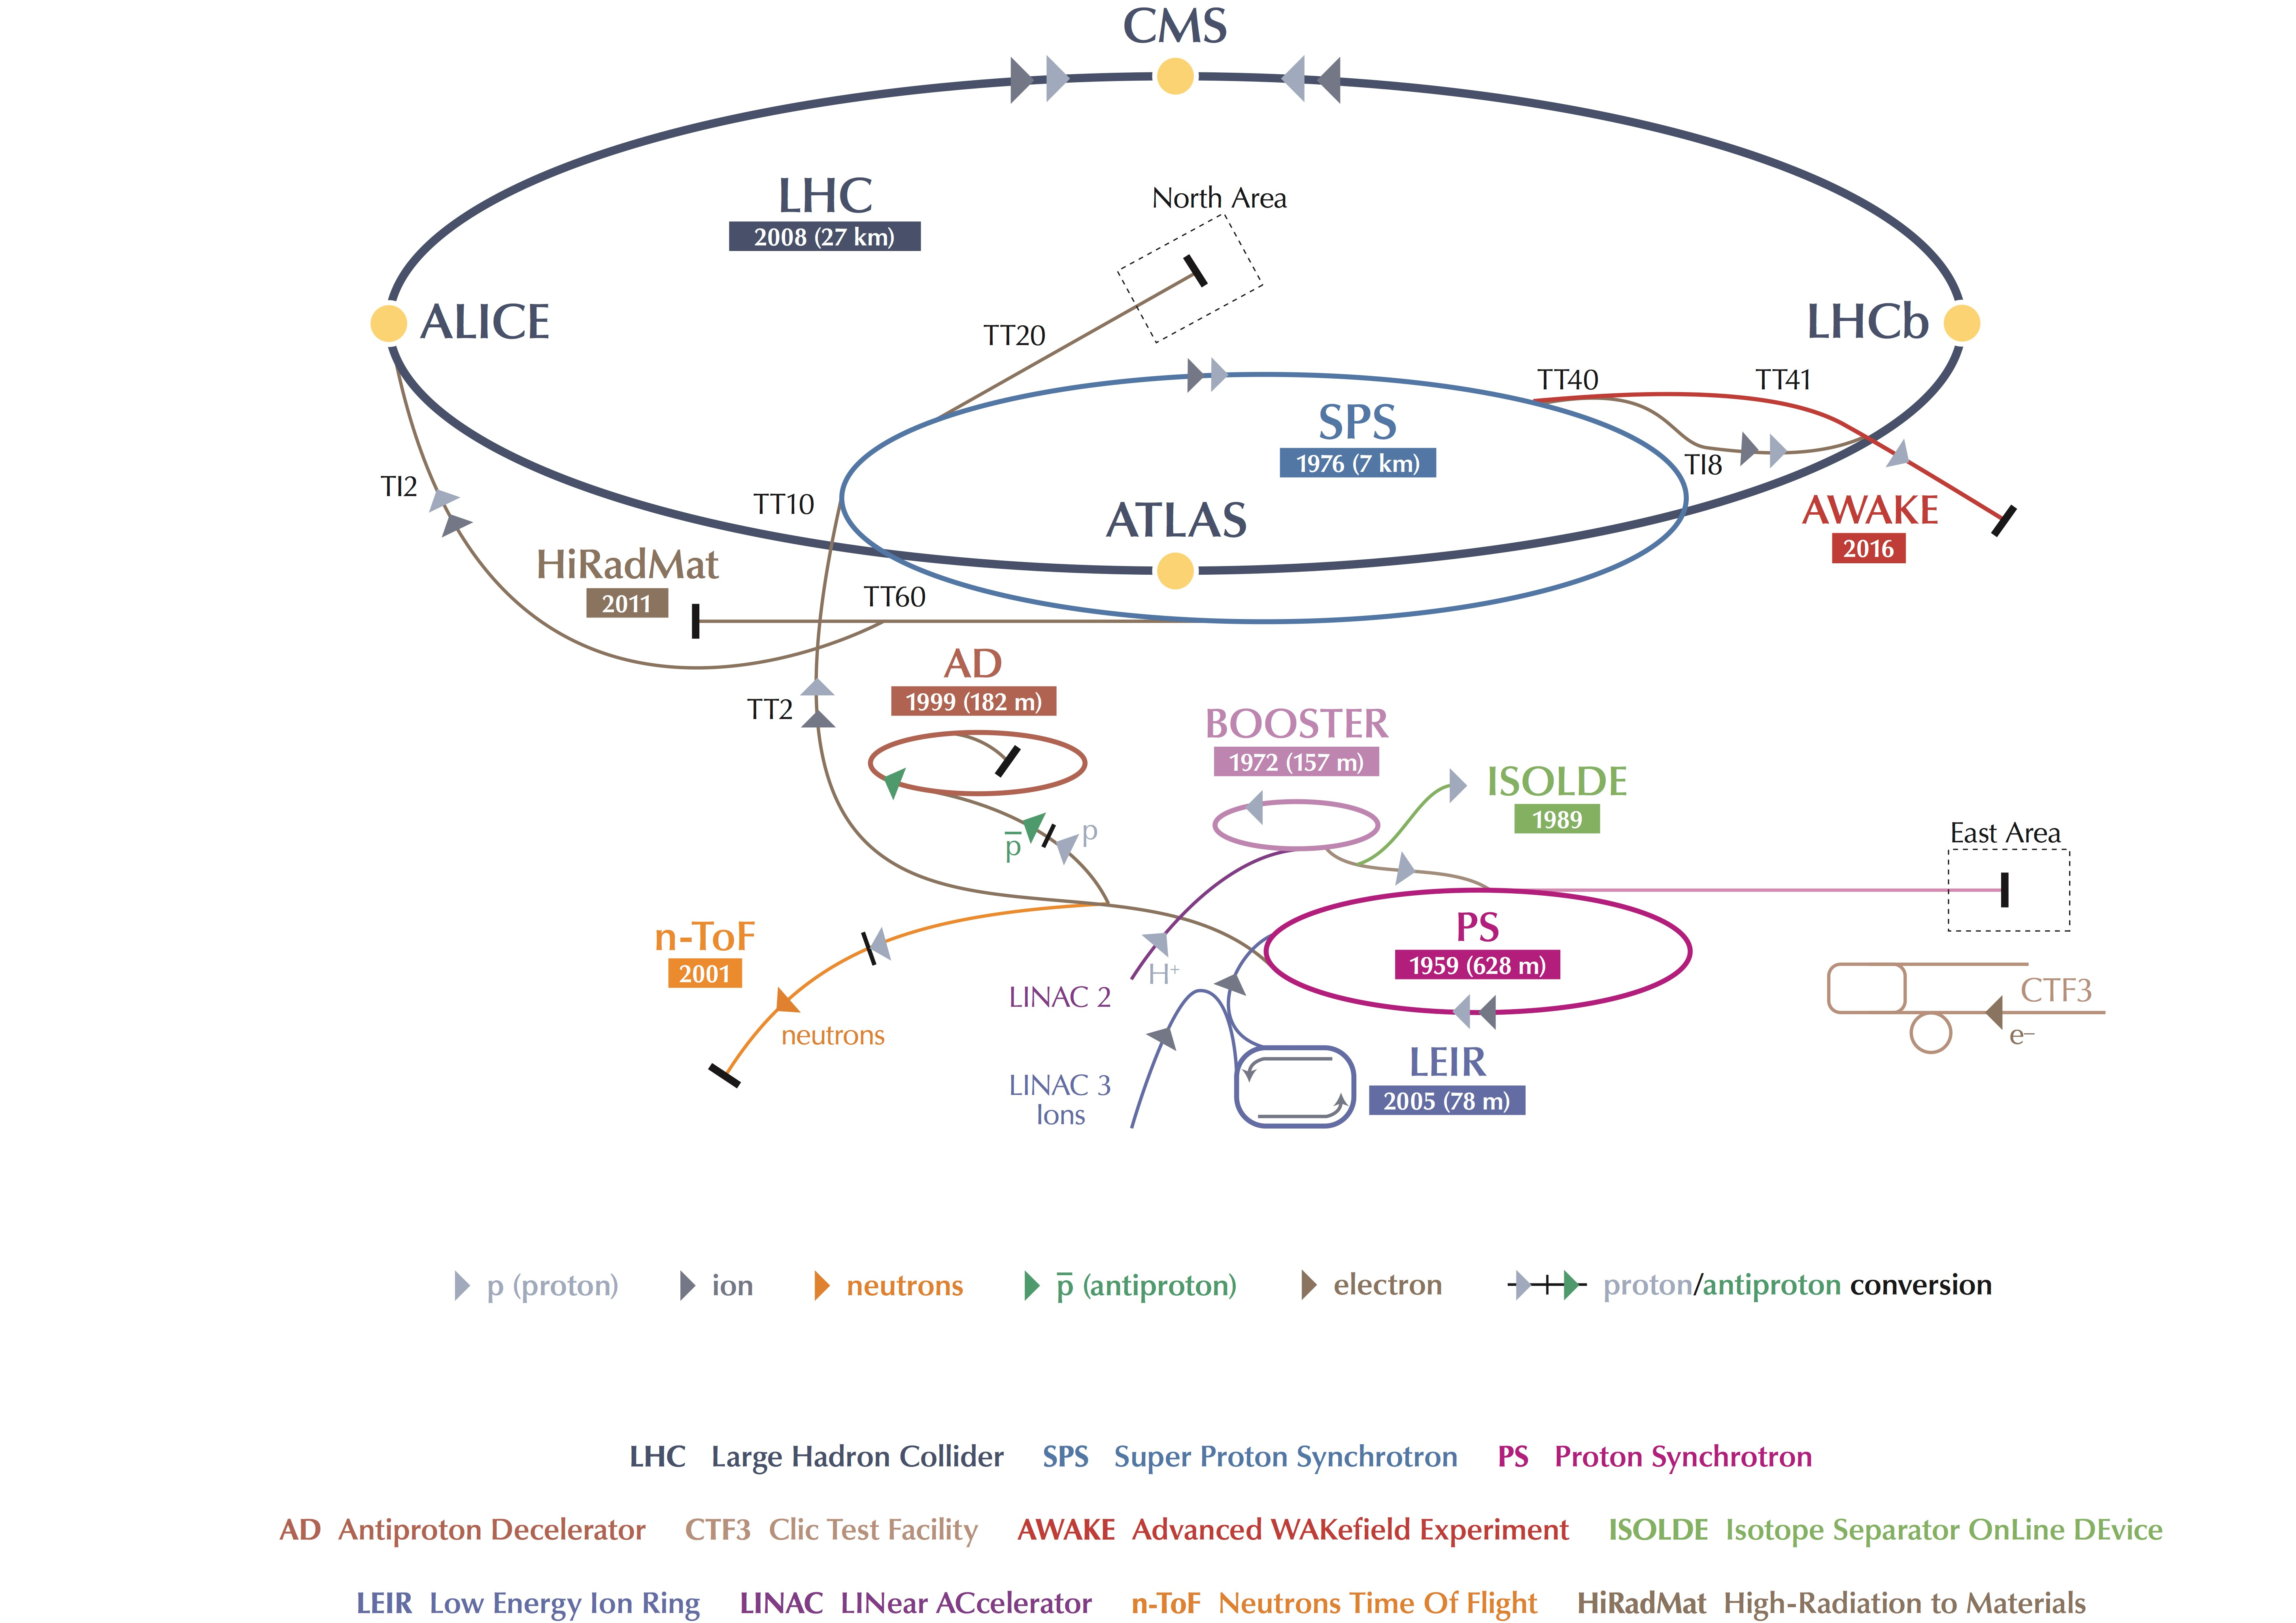
\includegraphics[width=\linewidth]{ExperimentalSetup/AcceleratorLayout_2.jpg}
\caption{A schematic of the accelerator chain.}
\label{fig:AcceleratorLayout}
\end{figure}

\section{The Compact Muon Solenoid Detector}
The Compact Muon Solenoid (CMS) detector is one of the general-purpose particle detectors at the LHC. It is made up of layered, sub-detectors arranged in a cylindrical structure that is 21.6 m long, 15 m in diameter and weighs about 14,000 tons. The detector is built around it’s huge solenoid magnet which provides a 3.8 T magnetic field. Due to the size of this magnet, the silicon tracker, the lead tungstate crystal electromagnetic calorimeter (ECAL), and the brass and plastic scintillator hadron calorimeter (HCAL) are all able to fit within the solenoid, allowing the momentum of particles to be precisely measured. Encasing the solenoid is the muon detector system composed of different types of gas-ionization detectors. A layout of the CMS detector can be seen in Figure~\ref{fig:CMSDetector}.

The experiment uses a right-handed, Cartesian coordinate system that is oriented with the x-axis pointing to the center of the LHC ring, the y-axis pointing up, and the z-axis pointing along the beam line. A pseudo-polar coordinate system is also used due to the cylindrical symmetry of the detector. The azimuthal angle, $\phi$, is measured from the x-axis in the x-y plane, the polar angle, $\theta$, is defined from the z-axis, and the pseudorapidity, $\eta$, is given by $\eta = -\mathrm{ln}\, \mathrm{tan}(\theta/2)$. The transverse plane is used to define the component of observable quantities, like momentum and energy, that is perpendicular to the beamline in the x-y plane. 

\begin{figure}[htbp]
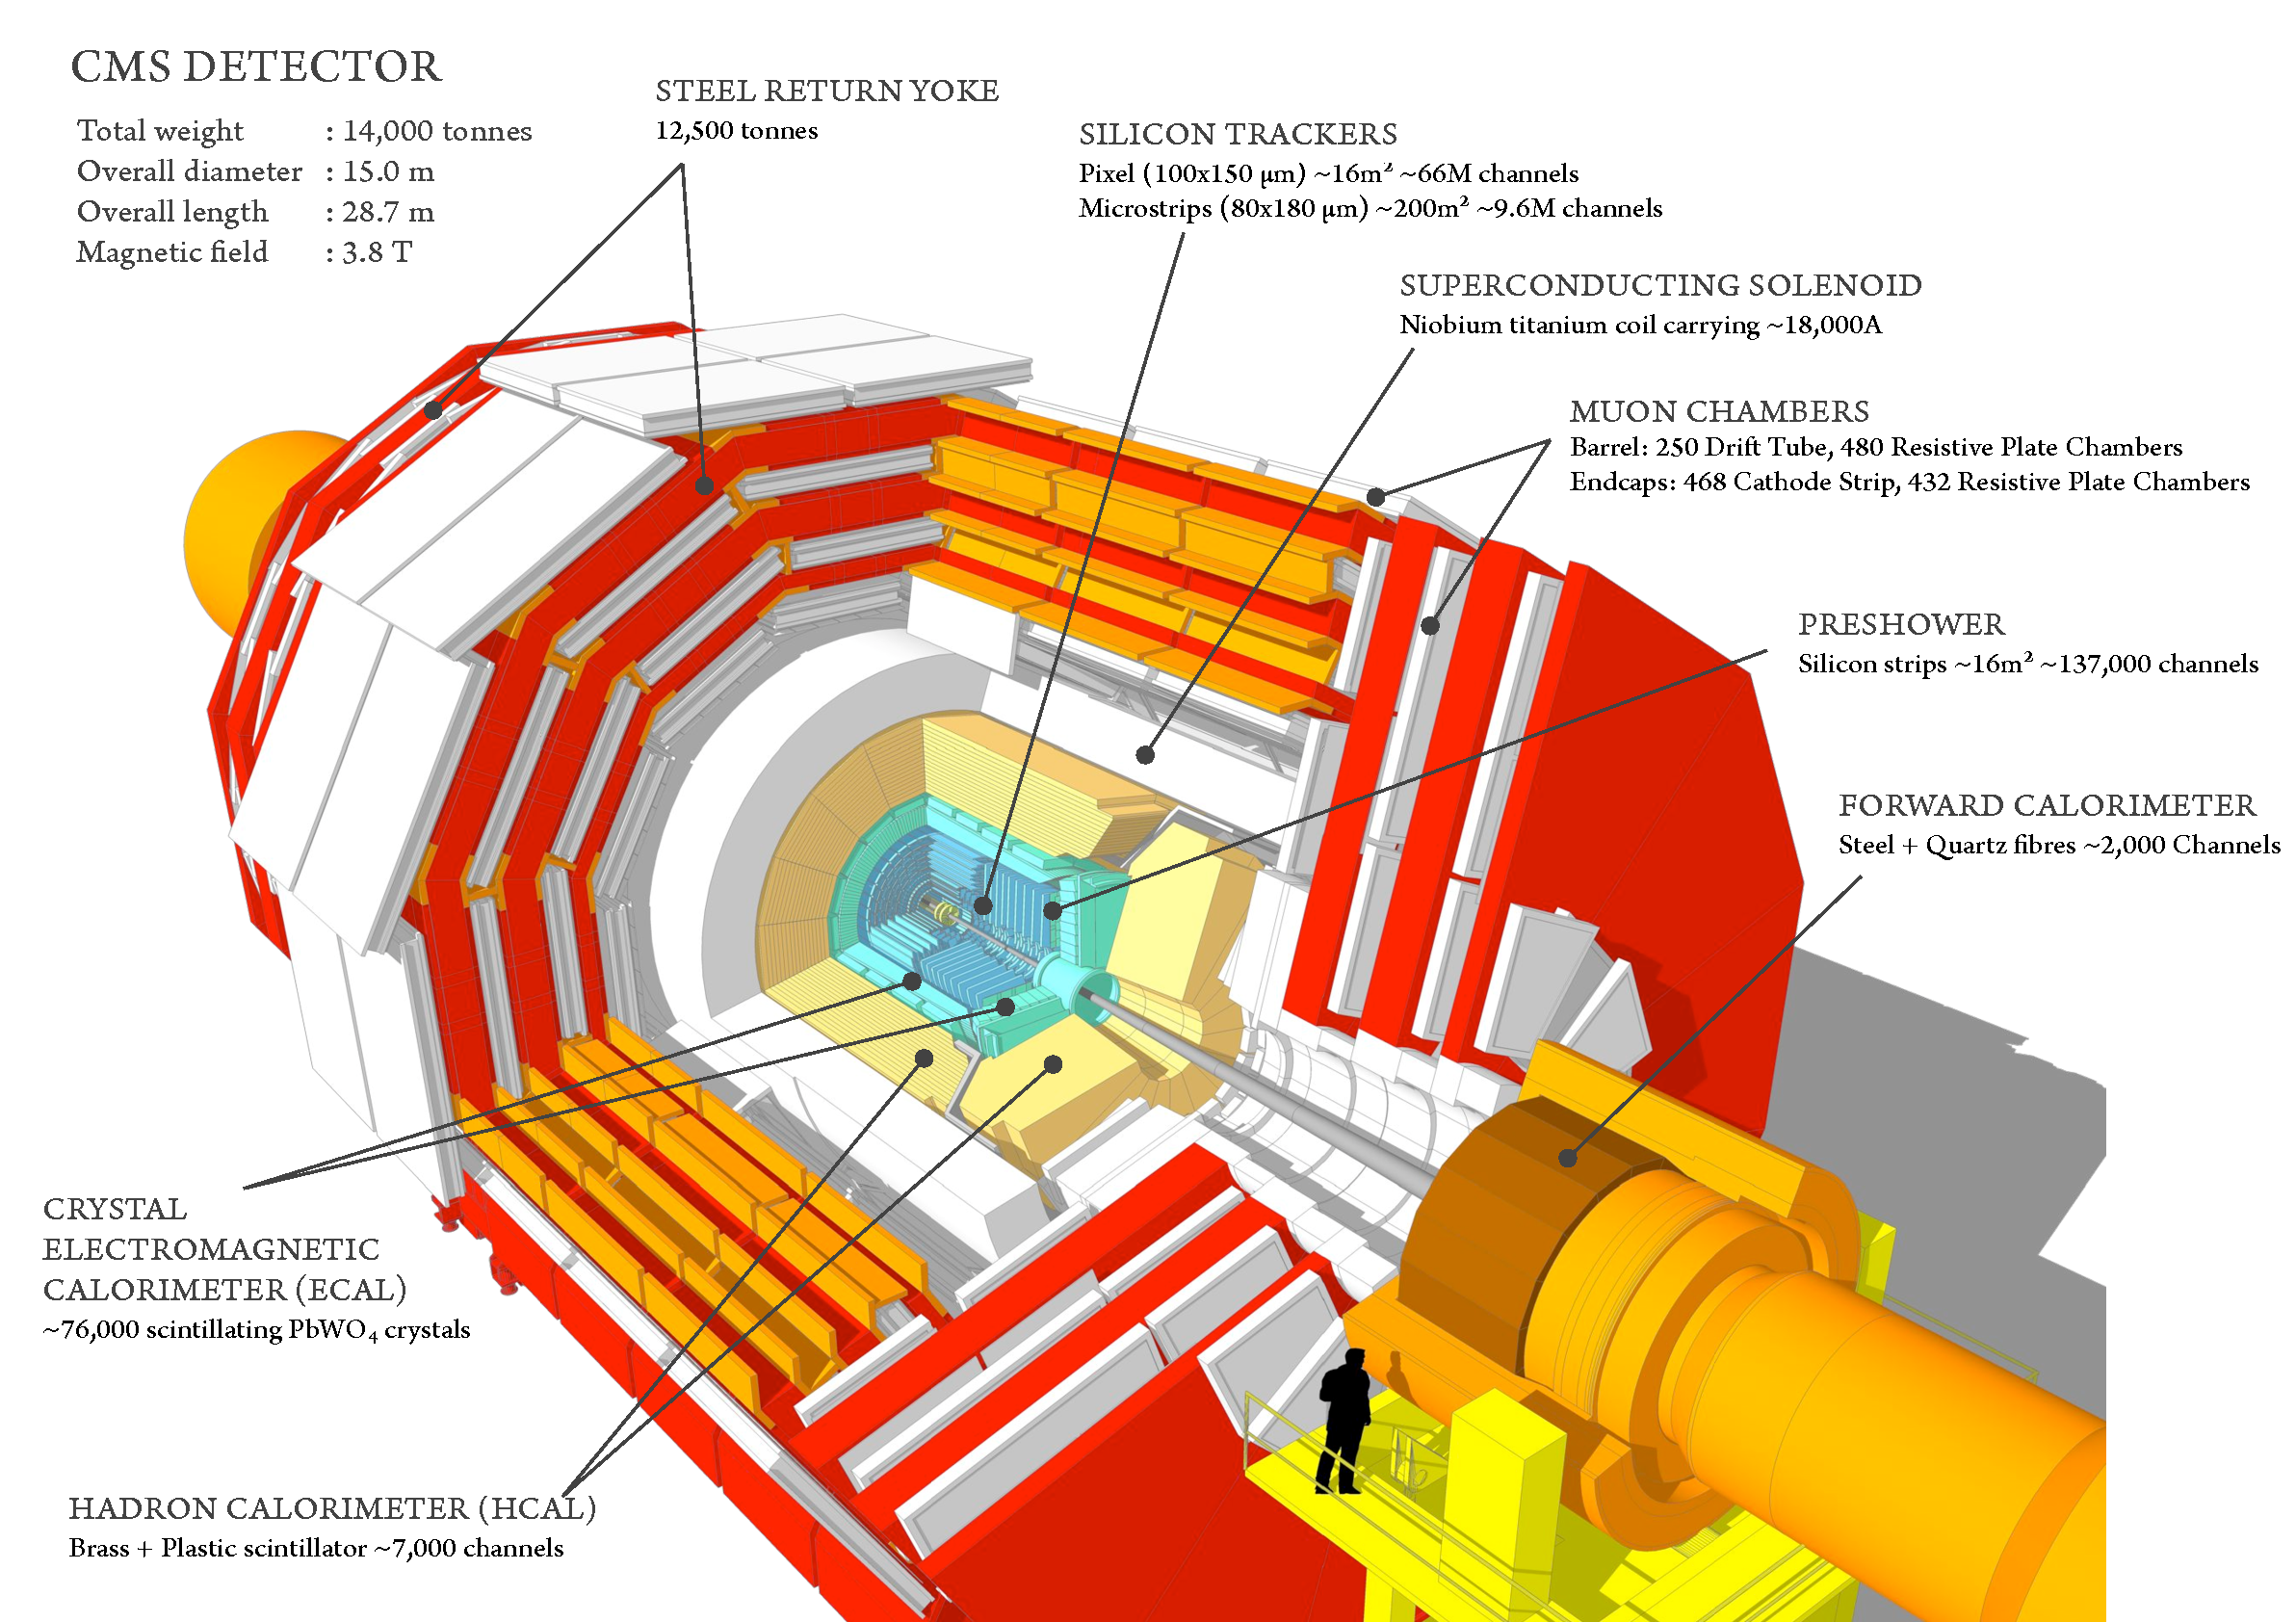
\includegraphics[width=\linewidth]{ExperimentalSetup/CMSDetector.png}
\caption{A sliced view of the CMS detector.}
\label{fig:CMSDetector}
\end{figure}

\subsection{The Tracker}
The tracker is the innermost layer of the CMS detector and is completely made of silicon. It consists of 2 separate subdetectors: the inner pixel detector and the outer strip detector. The purpose of the tracker is to collect precise, three-dimensional single hit positions along the curved trajectories of charged particles to extract their momentum. The tracker covers up to a pseudorapidity of $\mid\eta\mid < 2.5$. A schematic of the tracker can be seen in Figure~\ref{fig:CMSTracker}~\cite{CMSExperiment}. 

\begin{figure}[htbp]
\begin{center}
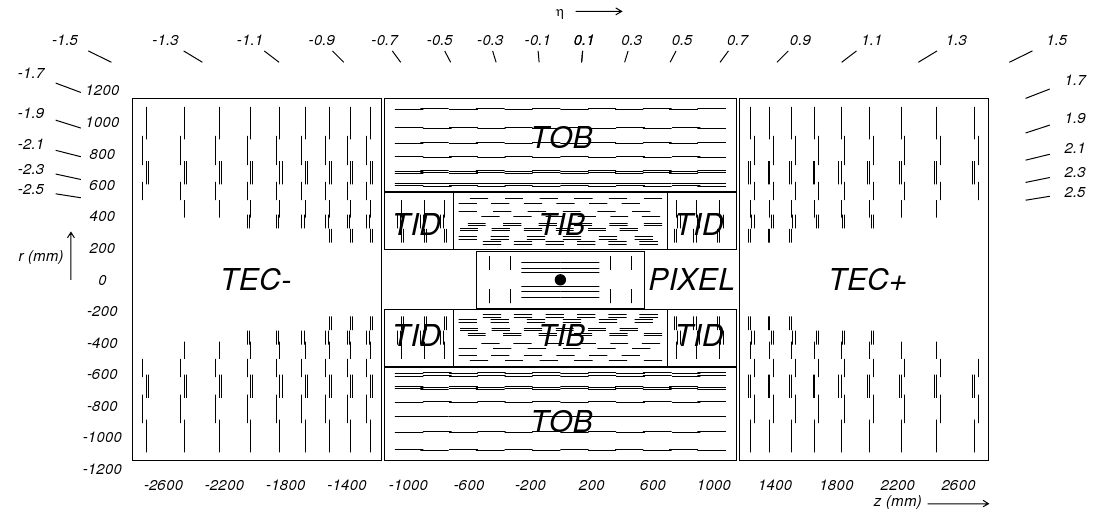
\includegraphics[width=120mm]{ExperimentalSetup/Tracker.png}
\end{center}
\caption{A schematic of the CMS tracker in the r-z plane.}
\label{fig:CMSTracker}
\end{figure}

\subsubsection{The Pixel Detector}
The pixel detector contains 65 million pixels that are $100 \times 150\,\mathrm{\mu m}^2$ with a thickness of $285\,\mathrm{\mu m}$. These pixels are contained in two different sections: the barrel (BPIX) and the endcaps (FPIX). The barrel is a cylindrical structure that surrounds the interaction vertex and consists of three concentric layers. These layers are at distances of 4.4, 7.3, and 10.2 cm from the beamlines. The endcap section consists of 2 symmetrical disk sections on either end of the barrel. Each section is made up of 2 disks that are 34.5 and 46.5 cm from the interaction point. At the end of the 2016 data taking period, an additional layer was added to the barrel region and the layers are now at distances of 3.0, 6.8, 10.2, and 16.0 cm. An additional disk was also added to each endcap region and each disk now consists of 2 concentric rings, inner and outer, to enable easy replacement.  A comparison of the 2016 and 2017 pixel detector geometries can be seen in Figure~\ref{fig:PixelUpgrade}\cite{CMSTracker}. 

\begin{figure}[htbp]
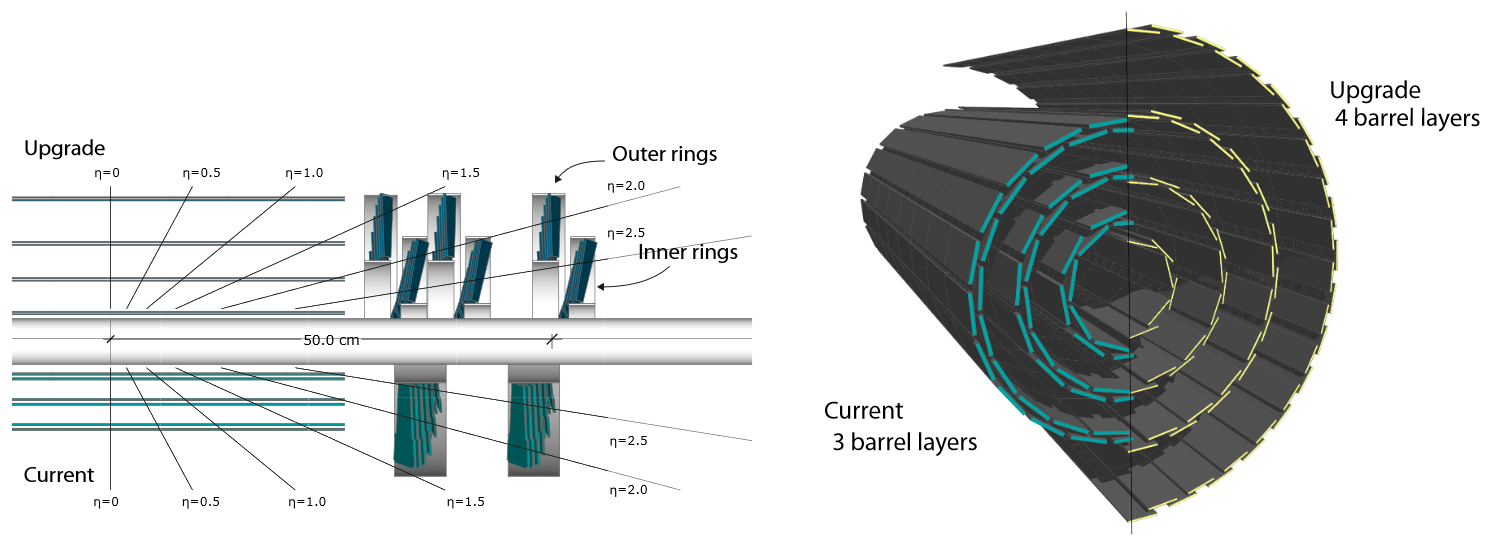
\includegraphics[width=\linewidth]{ExperimentalSetup/PixelDetectorUpgrade.png}
\caption{A comparison of the 2016 pixel detector geometry with the 2017 upgrade geometry.}
\label{fig:PixelUpgrade}
\end{figure}

The silicon pixels are grouped in modules of $52 \times 80$ pixels and bump-bonded to a read-out-chip (ROC). These ROCs amplify and shape the signals from the pixel sensors so that they can be converted from analog to digital signals.  

Due to the proximity of the pixel detector to the interaction point, the sensors and readout electronics will receive an incredibly high particle flux. The 
innermost layer of the BPIX is expected to receive a radiation dose of 840 kGy after an integrated luminosity of 500 $\mathrm{fb}^{-1}$.  A radiation tolerant design was a top priority for both the electronics and sensors and more details on this will be given in Chapter~\ref{RadiationStudies}.


\subsubsection{The Strip Detector}

Outside of the pixel detector is the strip detector which is arranged in a similar manner as the pixel detector. There is a barrel region that is split into an inner barrel (TIB) section and an outer barrel (TOB) section and two endcap sections on either side that consist of an inner endcap region (TID) and an outer endcap region (TEC). The TIB consists of four concentric cylinders that extend out to 65 cm on either side of the interaction point and have radii between 25.5 and 49.8 cm. The two inner layers are comprised of double sided modules with a strip pitch of 80 $\mu$m and the two outer layers are made of single sided modules with a strip pitch of 120 $\mu$m. The TOB consists of 6 concentric cylinders that extend from $-110$ to $+110$ along the z axis and are between radii of 55.5 to 116.0 cm. Each TID consists of 3 disks located between z = $\pm 80$ cm and z = $\pm$ 90 cm. A disk consists of 3 rings which span radii from 20 to 50 cm. The 2 innnermost rings have double sided modules and the outermost has single sided ones. The TEC disks extend radially from 22 to 113.5 cm and are located between $\pm$ 124 cm and $\pm$ 280 cm along the z direction. The silicon sensors in the TIB, TID, and inner 4 rings of the TEC are 320 $\mu$m thick and the sensors in the TOB and 3 outer rings of the TEC are 500 $\mu$m thick\cite{CMSExperiment}.

\subsection{The Electromagnetic Calorimeter}

Surrounding the tracker is the electromagnetic calorimeter (ECAL) which measures the energies of electrons and photons. The ECAL is made up of lead tungstate (PbWO4) crystals which produce scintillation light in fast, well defined photon showers whenever an electron or photon passes through them. These showers can be measured by photodetectors to determine the energy of the electron or photon. Since the yield of light in the crystals depends on temperature, the temperature of the ECAL does not vary by more than $0.1^{\circ}$C. 

The ECAL is made up of a barrel region which consists of 61,200 crystals and 2 endcap segments which consist of 7,324 crystals. The barrel covers a pseudorapidity of $|\eta| < 1.479$ and is made of crystals with a cross section of $22\times22\;\mathrm{mm}^{2}$ and a length of 230 mm, which corresponds to 25.8 radiation lengths. The photodetectors in the barrel region are avalanche photodiodes and are made of silicon. The endcaps cover a pseudorapidity of $1.48 < |\eta| < 3.0$ and the crystals have dimensions $24.7\times24.7\times220\;\mathrm{mm}^{3}$. The crystals are organized into groups of 36 crystals, called a supercrystal, and each endcap contains 268 supercrystals. The photodiodes in the endcaps are vacuum phototriodes and are used because of the higher radiation tolerance that is needed in this region.

Another component of the ECAL is the preshower detector. The preshower sits in front of both endcaps and covers a pseudorapidity of $1.65 < |\eta| < 2.61$. The purpose of the preshower is for extra spatial precision in order to distinguish single photons from a $\pi^{0}$ decaying to two nearby photons. The preshower is made of 2 planes of lead followed by silicon sensors that have dimensions of $6.3\;\mathrm{cm}\times6.3\;\mathrm{cm}\times0.3\;\mathrm{mm}$\cite{CMSExperiment}\cite{CMSECAL}. 

The layout of the ECAL can be seen in Figure~\ref{fig:ECALSchematic}.

\begin{figure}[htbp]
\begin{center}
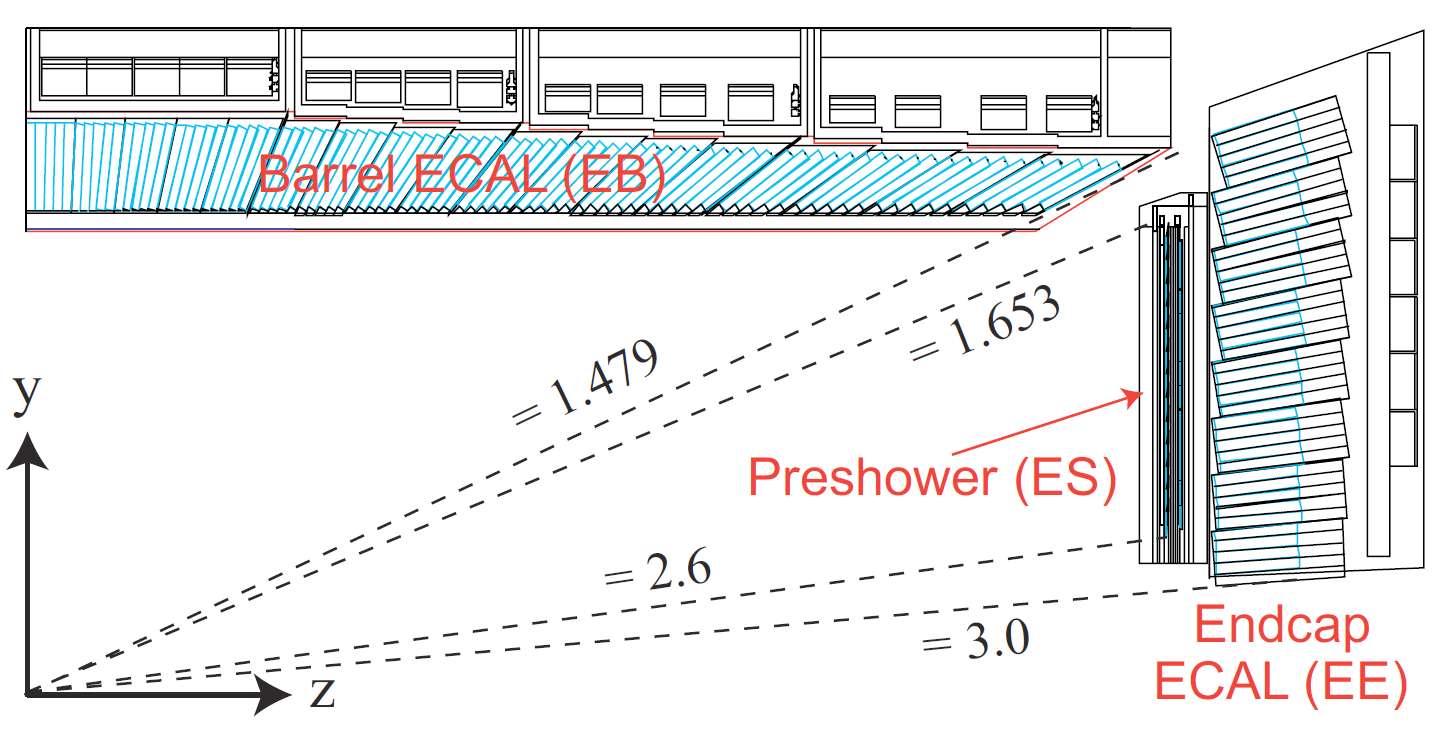
\includegraphics[width=140mm]{ExperimentalSetup/ECAL_Layout.png}
\end{center}
\caption{Schematic view of a quadrant of the electromagnetic calorimeter (ECAL). The numbers correspond to $\eta$ and show the coverage of the different sections of the ECAL.}
\label{fig:ECALSchematic}
\end{figure}

\subsection{The Hadron Calorimeter}

The hadron calorimeter (HCAL) surrounds the ECAL and its purpose is to measure the energy of hadrons. It is designed to be a hermetic detector because all particles from an interaction must be detected to accurately measure the missing transverse energy (MET) of an event. The HCAL is a sampling detector that is made up of alternating layers of absorber and scintillator. The absorbers are made of either brass or steel and when a particle hits them a shower of particles is produced. Light is then emitted when particles pass through the scintillation material and absorbed by wavelength-shifting fibers that are less than 1 mm in diameter. The HCAL is divided into 4 sections: the barrel (HB), the endcap (HE), the outer calorimeter (HO), and the forward calorimeter (HF). A schematic of the HCAL can be viewed in Figure~\ref{fig:HCALSchematic}\cite{CMSExperiment}.

\begin{figure}[htbp]
\begin{center}
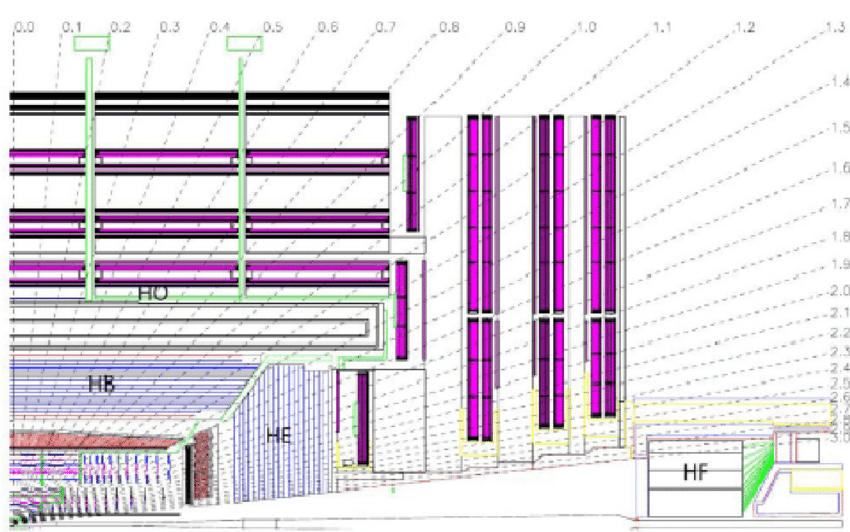
\includegraphics[width=130mm]{ExperimentalSetup/HCAL_Layout4.png}
\end{center}
\caption{Schematic cross section of the hadron calorimeter (HCAL).}
\label{fig:HCALSchematic}
\end{figure}

The HB sits inside the magnet and covers a pseudorapidity of $|\eta| < 1.3$. It is made up of 36 wedges aligned parallel to the beam axis, where each wedge consists of brass plates interspersed by plastic scintillator. The plastic scintillator plates are divided into 16 sections giving a granularity of $\Delta\eta \times \Delta\phi = 0.087 \times 0.087$. For structural support, the outermost layers of each wedge are steel plates.

The HE is designed to sustain a high radiation flux due to the pseudorapidity region it covers, $1.3 < |\eta| < 3$. It also must provide the maximum number of interaction lengths to contain hadronic showers. Thus, C26000 brass was chosen as the absorber and the combined material in the HE provides about ten interaction lengths. For $|\eta| < 1.6$ the granularity is $\Delta\eta \times \Delta\phi = 0.087^{2}$ while for $|\eta| >= 1.6$ the granularity is $\Delta\eta \times \Delta\phi = 0.17^{2}$. 

Due to the limited space within the solenoid magnet, the HO sits outside of the magnet and detects any late starting showers. The HO covers $|\eta| < 1.3$ and adds more material to the barrel region to provide 11.8 radiation lengths. Since the HO detects energy that would otherwise be missed, it improves missing transverse energy (MET) measurements.

 The HF sits 11.2 m from the interaction point down the beam line. It is a cylindrical structure with an outer radius of 130 cm. Due to the extreme, 760 GeV energy per proton-proton interaction deposited into the forward calorimeters, quartz fibers are used as the active medium. It has a granularity of $\Delta\eta \times \Delta\phi = 0.175\times 0.175$ and covers a pseudorapidity range of $3.0 < |\eta| < 5.0$.

\subsection{The Superconducting Magnet}

As implied by the name of CMS, the superconducting magnet is a central design feature of the detector. By producing a uniform, 3.8 T magnetic field the paths of charged particles are bent and the momentum of these particles can be accurately measured. The magnet is a solenoid with a length of 12.5 m and a 6.3 m inside diameter. This large space allows the tracker, ECAL and HCAL to fit inside the solenoid. The magnet is made up of 4-layers of NbTi wires that are coiled and then cooled to $-268.5^{\circ}$C to allow electricity to flow through with minimal resistance and produce the largest magnetic field possible. The magnetic flux is returned through a yoke that weighs 10,000 tons and is made up of six endcap disks and five barrel wheels.

\subsection{The Muon System}

The muon system is the outermost sub-detector of CMS since muons have a small cross section and can pass through several meters of iron without interacting. There are 1400 muon chambers that compose the muon system and these chambers consist of three different types of detectors: drift tubes (DTs), cathode strip chambers (CSCs), and resistive plate chambers (RPCs). The muon system sits between the magnet return yolk and covers a pseudorapidity of $|\eta| < 2.4$. The DTs and RPCs make up the barrel region of the sub-detector and the CSCs and RPCs make up the endcap regions. A detailed view of the muon system can be seen in Figure~\ref{fig:MuonSchematic}\cite{CMSExperiment}.

\begin{figure}[htbp]
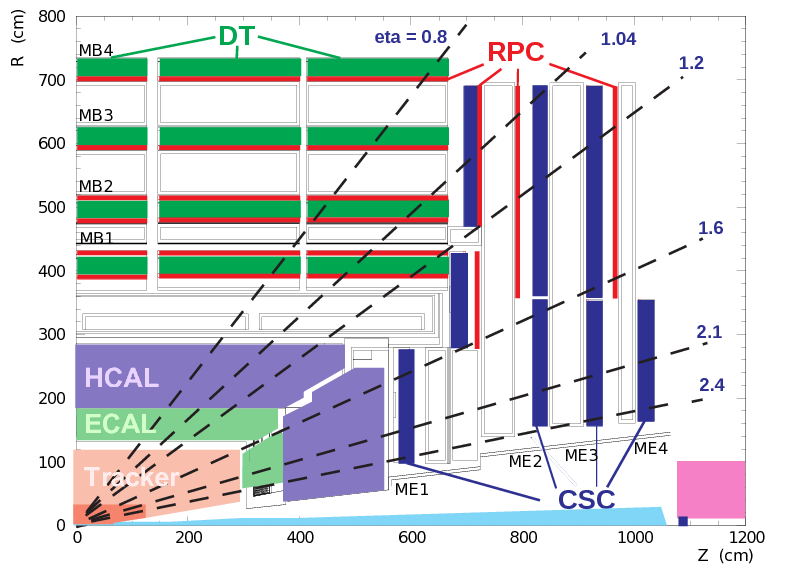
\includegraphics[width=\linewidth]{ExperimentalSetup/MuonLayout.png}
\caption{Schematic view of the muon system.}
\label{fig:MuonSchematic}
\end{figure}

The DTs are 4 cm wide tubes that contain a wire within a gas volume comprised of $85\%$ Ar and $15\%$ $\mathrm{CO}_{2}$. The muons knock electrons off the atoms of the gas and collect on the wire where a positive voltage is applied. The drift velocity of electrons in the gaseous mixture is known and thus two position coordinates can be measured. The DTs are arranged in 4 concentric cylinders around the beamline and cover a pseudorapidity of $|\eta| < 1.2$. 

CSCs are made of arrays of positively charged anode wires crossed with negatively charged cathode strips within a gas volume. Electrons from the interacting muons are detected in a similar way as the DTs and since the wires and strips are perpendicular to each other 2 position coordinates are measured. The CSCs cover the pseudorapidity range $0.9 < |\eta| < 2.4$ and are arranged in 5 separate layers that are made up of different numbers of rings.

RPCs are made of 2 oppositely charged parallel plates that are made of a high resistivity plastic material and separated by a gaseous volume. The plates are transparent to electrons which are detected by external metallic strips. The RPCs give a coarser resolution than the DTs and CSCs, but have a timing resolution on the order of nanoseconds. They cover $|\eta| < 1.6$ and are primarily used as a secondary muon identification tool to confirm the measurements in the DTs and CSCs. 

%At 1 TeV the standalone momentum resolution varies between $15\%$ and $40\%$ depending on $|\eta|$. $9\%$ resolution for muons up to 200 GeV. Including the tracker improves resolution by an order of magnitude for muons below 200 GeV.


\subsection{The Trigger System}

Collisions at CMS occur every 25 ns or at a rate of 40 MHz, which is an impossible amount of data to store. To reduce the amount of data, CMS employs a trigger system that attempts to only save interesting events. To do this, the trigger system is made up of 2 triggers: the Level-1 (L1) trigger and the high level trigger (HLT). The L1 trigger consists of programmable electronics and reduces the rate to 100 kHz. The HLT uses software to reconstruct physics objects and reduces the rate to below 1 kHz. 

\subsubsection{The Level-1 Trigger}

The L1 trigger uses information from every sub-detector, except for the tracker, to determine whether an event is passed to the HLT. It has a 3.2 $\mu$s latency period to make this decision and the tracker cannot provide information from its measurements in this small time frame.  The final step of the L1 trigger that decides whether an event is kept or rejected is the Global Trigger and it uses information from the calorimeter trigger and muon trigger to make this decision.

The initial step of the calorimeter trigger is the Trigger Primitive Generators (TPG), which sum the transverse energies measured in ECAL crystals or HCAL read-out towers. This info is used to determine possible electrons or photons, transverse energy sums, and tau-veto bits by the Regional Calorimeter Trigger. The Global Calorimeter Trigger then determines the highest-rank calorimeter trigger objects across the entire detector. It determines jets, total transverse energy, MET, jet counts, HT, and the highest-rank isolated and non-isolated electron and photon candidates.

%The muon trigger uses track segments in the $\phi$-projection and hit patterns in the $\eta$-projection from the DT chambers. CSCs provide 3-dimensional track segments. The Regional Muon Triggers consists of the DT and CSC Track Finders, which join segments to complete tracks. RPC chambers provide their own track candidates based on regional hit patterns. The Global Muon Trigger combines info from the 3 sub-detectors to improve the momentum resolution and efficiency.

The muon trigger uses track segments combined from the DTs and CSCs, as well as separate track candidates from the RPCs. The Global Muon Trigger combines this information to achieve the best momentum resolution and efficiency possible and determine the four best muon candidates.
 
The architecture of the L1 trigger system can be seen in Figure~\ref{fig:L1Trigger}.

\begin{figure}[htbp]
\begin{center}
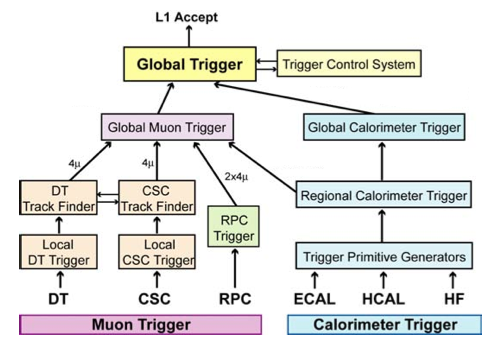
\includegraphics[width=120mm]{ExperimentalSetup/L1Trigger.png}
\end{center}
\caption{Schematic of the Level-1 trigger system.}
\label{fig:L1Trigger}
\end{figure}

\subsubsection{The High Level Trigger}

The HLT is a software based system that uses reconstructed physics objects to make complicated calculations. These calculations are done using similar software to what is used in offline analyses. The HLT is made up of many different HLT paths that are implemented for specific analyses and each consist of a sequence of steps of reconstructing and filtering in increasing complexity. 



%%\section{\centering Experimental Setup}
\chapter{Object Reconstruction}
%\chapter*{\centering Experimental Setup}
\label{ch:ObjReco}

The CMS detector attempts to identify all particles produced from proton-proton collisions. However, all the information from an event is provided as hit patterns in the subdetectors and for these hit patterns to be analyzed they must be converted into physics objects. This chapter will describe the Particle Flow algorithm used by CMS to reconstruct all stable particles: electrons, muons, photon, charged and neutral hadrons. 

\section{The Particle Flow Algorithm}

The Particle Flow (PF) algorithm~\cite{PFAlgorithm, PFReconstruction} optimally combines information from all the subdetectors to identify and reconstruct every individual particle coming from a proton-proton (pp) collision. To accomplish this, the CMS detector was designed with excellent calorimeter granularity to disentangle overlapping showers and a nearly fully efficient tracking system to precisely reconstruct tracks and vertices. The PF algorithm is comprised of three main elements: iterative tracking, calorimeter clustering, and the link algorithm.

\subsection{Iterative Tracking}

To reconstruct the charged particles from a pp collision, the hits in the tracker need to be converted into a collection of tracks. The tracking software used by the PF algorithm is called the Combinatorial Track Finder (CFT)~\cite{TrackReco} and it allows pattern recognition and track fitting to occur in the same framework. The CFT is run six times with the reconstruction criteria loosening for each iteration to achieve both a high efficiency and low fake rate. Each iteration is comprised of four steps: seed generation, track finding, track fitting, and track selection.

Seed generation determines initial track trajectories from the minimum number of hits needed to define a trajectory in a magnetic field. Five parameters are needed to define a helical trajectory and thus, either 3 hits or 2 hits and an additional constraint that the particle originates from the beam spot are used to define the seeds. These seeds are required to pass some minimum $p_{T}$ threshold and must be consistent with originating from the proton-proton interaction region. Next, the initial track trajectories are extrapolated out and at each detector layer the hit with the smallest $\chi^{2}$ to the trajectory is added to the track. This process is repeated at each detector layer until the end of the tracker is reached. When there is no hit along the trajectory at a certain layer a ``ghost'' hit is added to the track. Tracks are discarded after a certain amount of ghost hits are recorded. To obtain the full information of the trajectory, tracks are refitted with all hits using a Kalman filter and smoother~\cite{KalmanFilter}. Finally, tracks are selected if they pass a certain amount of quality requirements such as the number of layers with hits, the $\chi^{2}/\mathrm{ndf}$ of the track fit, and the compatibility that the track originates from the primary vertex. This greatly reduces the number of fake tracks. 

%To define a trajectory in a magnetic field, five parameters are needed and thus seed generation uses 3 hits in the tracker or 2 hits in the tracker and an additional constraint that the particle originates from the beam spot to define initial trajectories. 

%These seeds are required to pass some minimum $p_{T}$ threshold and must be consistent with originating from the proton-proton interaction region. Next, the initial track trajectories are extrapolated out and at each detector layer the hit with the smallest $\chi^{2}$ to the trajectory is added to the track. This process is repeated at each detector layer until the end of the tracker is reached. When there is no hit along the trajectory at a certain layer a “ghost” hit is added to the track. Tracks are discarded after a certain amount of ghost hits are recorded. To obtain the full information of the trajectory, tracks are refitted with all hits using a Kalman filter and smoother~\cite{KalmanFilter}. Finally, tracks are selected if they pass a certain amount of quality requirements such as the number of layers with hits, the $\chi^{2}/ndf$ of the track fit, and the compatibility that they originate from the primary vertex. This greatly reduces the number of fake tracks. 

\subsection{Calorimeter Clustering}

There are four purposes to the clustering algorithm in the calorimeter: detect and measure the energy and direction of neutral particles, separate these neutral particles from energy deposits of charged ones, reconstruct and identify electrons and all accompanying Bremsstrahlung photons, and assist the energy measurement of charged hadrons when track parameters aren’t accurately determined. The clustering algorithm is therefore designed for a high detection efficiency for low-energy particles and a separation of close energy deposits from the high granularity calorimeter. Clustering is performed separately in each subdetector as follows.

First, the seed for a cluster of nearby hits is identified as the hit with the maximum energy. Then topological clusters are created by adding cells that are adjacent to the seed. Finally, the final energy and position of the cluster is determined through an iterative procedure. 

\subsection{The Link Algorithm}

The purpose of the link algorithm is to connect the different PF elements from the subdetectors to fully reconstruct a particle. The elements that can be linked are charged-particle tracks, calorimeter clusters, and muon tracks. The link algorithm creates blocks of elements which contain two or three elements. 

A link between a track and a calorimeter cluster is made if the extrapolated track from the tracker lands within the cluster. Clusters from different calorimeter subdetectors are linked when the position in the more granular calorimeter is within the cluster envelope in the less granular calorimeter. And finally, links between tracker tracks and muon tracks are made when a global fit of the combied tracks returns an acceptable $\chi^{2}$. 

\subsection{Particle Identification}

Each block of elements is then identified as specific particles in the following way. First, muons are identified when the momentum of the global muon is within $3 \sigma$ of the tracker momentum. The corresponding tracks are then removed from the block. Secondly, electrons are identified by finding tracks that fit the criteria of an electron track: short tracks that lose energy from Bremsstrahlung. These tracks are refit with a Gaussian-Sum fitter~\cite{GausSumFilter} to follow their trajectories out to the ECAL. The corresponding track and ECAL cluster are then removed from the block. Thirdly, charged hadrons are identified from the remaining tracks and are associated to clusters in the HCAL if the cluster energy falls within the uncertainties of the track momentum. Finally, the remaining clusters in the HCAL and ECAL are associated with neutral hadrons and photons, respectively. 

\section{Vertex Reconstruction}

The purpose of vertex reconstruction is to measure the location of all proton-proton interactions within an event. It consists of three steps: track selection, clustering tracks originating from the same vertex, and fitting the tracks for the position of each vertex. 

Track are selected that are produced promptly in the primary interaction region. This is done by placing requirements on the impact parameter off the track relative to the center of the beam, the number of hits within the track, and the $\chi^{2}$ of the fit trajectory. The tracks are then clustered according to their z-coordinate at their point of closest approach to the center of the beam spot. Finally, the position of each vertex is determined by fitting each cluster of tracks~\cite{TrackReco}. 

\section{Jet Reconstruction}
In an attempt to reconstruct the hadronization of a quark or gluon, the hadrons and non-isolated leptons of an event are clustered together to form jets, which is a cone surrounding the initial quark or gluon. In this analysis, the ``anti-$k_{t}$'' algorithm is used to create jets. This algorithm iteratively clusters particles together by defining two distance parameters
%distance between particles $i$ and $j$ as

\begin{equation}
d_{ij}=min(k_{ti}^{2p},k_{tj}^{2p})\frac{\Delta_{ij}^{2}}{R^{2}}
\end{equation}
\begin{equation}
d_{iB} = k_{ti}^{2p}
\end{equation}
where $k_{ti}$ is the transverse momentum of particle $i$, $\Delta_{ij}^{2} = (y_{i}-y_{j})^{2}+(\phi_{i}-\phi_{j})^{2}$, $y_{i}$ is the rapidity, $\phi_{i}$ is the azimuth, R is the chosen cone radius, and $p=-1$ gives the anti-$k_{t}$ algorithm. The distance between particles $i$ and $j$, $d_{ij}$, is compared to $d_{iB}$, the distance between particle $i$ and the beam. If $d_{ij}$ is smaller than $d_{iB}$ then $i$ and $j$ are recombined, but if $d_{ij}$ is larger then $i$ is called a jet and removed from the remaining particles. This continues until are particles have been clustered into jets.

The anti-$k_{t}$ algorithm clusters low $p_{T}$, or soft, particles to high $p_{T}$, or hard, ones, so that a jet's axis is mainly defined by it's hard constituents. This is a key feature of this algorithm because the jet's axis will not dramatically change when soft radiation from pileup is removed from the event. When two hard particles are nearby, they are either clustered together or the soft particles are shared between them based on the size of the cones being reconstructed. 

\section{Missing Transverse Energy}

The initial momentum of the colliding protons at CMS is unknown, however it is known that their transverse momentum is zero. Therefore, by conservation of momentum, the combined transverse momentum of all of the particles produced in the collision is zero. However, weakly interacting particles, like neutrinos, can avoid detection and cause there to be an imbalance in the transverse momentum of a collision. These signatures are predicted by many theoretical models and thus, a useful quantity in analysis of CMS data is the missing transverse momentum:

\begin{equation}
\vec{\cancel{E}_{T}}= -\sum_{detected\;particles} \vec{p_{T}}
\end{equation}
This quantity is referred to as MET throughout this paper.




%\bibliographystyle{abbrv}
%\bibliography{Thesis}

%\end{document}
\documentclass[defaultstyle,11pt]{thesis}

\usepackage{amssymb}		% to get all AMS symbols
\usepackage{graphicx}		% to insert figures
\usepackage{hyperref}		% PDF hyperreferences??
\usepackage{cancel}
\usepackage{mhchem}
\usepackage{subcaption}
\usepackage{textcomp}
\usepackage{float}

%%%%%%%%%%%%   All the preamble material:   %%%%%%%%%%%%

\title{This is the Name of my Thesis}

\author{I.~B.}{Scriptor}

\otherdegrees{B.A., North Dakota State University, 2005 \\
	      M.S., University of Reno, 2007}

\degree{Doctor of Philosophy}		%  #1 {long descr.}
	{Ph.D., Rocket Science}		%  #2 {short descr.}

\dept{Department of}			%  #1 {designation}
	{Rocket Science}		%  #2 {name}

\advisor{Prof.}				%  #1 {title}
	{Ed Visor}			%  #2 {name}

\reader{Prof.~Rachel Goddard}		%  2nd person to sign thesis
\readerThree{Ms.~Thora Nea}		%  3rd person to sign thesis

\abstract{  \OnePageChapter	% because it is very short

	Often the abstract will be long enough to require
	more than one page, in which case the macro
	``$\backslash$OnePageChapter'' should {\it not}
	be used.

	But this one isn't, so it should.
	}

\dedication[Dedication]{	% NEVER use \OnePageChapter here.
	To all of the fluffy kitties.
	}

\acknowledgements{	\OnePageChapter	% *MUST* BE ONLY ONE PAGE!
	Here's where you acknowledge folks who helped.
	But keep it short, i.e., no more than one page,
	as required by the Grad School Specifications.
	}

% \IRBprotocol{E927F29.001X}	% optional!

\ToCisShort	% use this only for 1-page Table of Contents

\LoFisShort	% use this only for 1-page Table of Figures
% \emptyLoF	% use this if there is no List of Figures

\LoTisShort	% use this only for 1-page Table of Tables
% \emptyLoT	% use this if there is no List of Tables

\graphicspath{ {Thesis_Images/} }

%%%%%%%%%%%%%%%%%%%%%%%%%%%%%%%%%%%%%%%%%%%%%%%%%%%%%%%%%%%%%%%%%
%%%%%%%%%%%%%%%       BEGIN DOCUMENT...         %%%%%%%%%%%%%%%%%
%%%%%%%%%%%%%%%%%%%%%%%%%%%%%%%%%%%%%%%%%%%%%%%%%%%%%%%%%%%%%%%%%

\begin{document}

\input macros.tex
%\input Intro_Chapter.tex
%\input Theory_Chapter.tex
%\input ExperimentalSetup_Chapter.tex
%\input ObjectReconstruction_Chapter.tex
%\input RadiationStudies_Chapter.tex
\input Analysis_Chapter.tex

%%%%%%%%%   then the Bibliography, if any   %%%%%%%%%
\bibliographystyle{plain}	% or "siam", or "alpha", etc.
\nocite{*}		% list all refs in database, cited or not
\bibliography{Thesis}		% Bib database in "refs.bib"

%%%%%%%%%   then the Appendices, if any   %%%%%%%%%
\appendix
%\input appendixA.tex
%\input appendixB.tex


\end{document}

